

\clearpage

\section{M-QAM Transmitter}

\begin{tcolorbox}	
	\begin{tabular}{p{2.75cm} p{0.2cm} p{10.5cm}} 	
		\textbf{Header File}   &:& m\_qam\_transmitter.h \\
		\textbf{Source File}   &:& m\_qam\_transmitter.cpp \\
        \textbf{Version}       &:& 20190403 (\emph{Bruno Santos})\\
	\end{tabular}
\end{tcolorbox}
\begin{text}
This block simulates an QAM transmitter which has the ability to send multiple bits in one symbol, by modulating two orthogonal carriers in amplitude and conjugating info from both.
\end{text}

\subsection*{Signals}
\subsubsection{Inputs}
\subparagraph*{Number:} 0 Data In
\subparagraph*{Type:} Binary Signal
\bigbreak
\subsection{Outputs}
\subparagraph*{Number:} 8 Optical Signal Out
\subparagraph*{Type:} Optical Signal
\bigbreak
\subsubsection{Internal Signals}
\subparagraph*{Number:} 1 and 2 MQam Mapper Out (Quadrature and phase)
\subparagraph*{Type:} Electrical Signal
\bigbreak
\subparagraph*{Number:} 3 and 4 Discrete to Continuous Time Out(Quadrature and phase)
\subparagraph*{Type:} Electrical Signal
\bigbreak
\subparagraph*{Number:} 5 and 6 Pulse Shaper Out (Quadrature and Phase)
\subparagraph*{Type:} Electrical Signal
\bigbreak
\subparagraph*{Number:} 7 Tx Local Oscillator
\subparagraph*{Type:} Optical Signal
\bigbreak

\subsection*{Input parameters}

\begin{itemize}
    \item int constellationCardinality( 4 )
    \item double symbolPeriod\textunderscore s( 2e-11 )
    \item int samplesPerSymbol( 8 )
    \item double txLocalOscillatorPower\textunderscore dBm( 0 )
    \item pulse\textunderscore shapper\textunderscore filter\textunderscore typetxPulseShapperType( pulse\textunderscore shapper\textunderscore filter\textunderscore type)
    \item double raisedCosineRollOffFactor( 0.1 )
    \item int txPulseShaperLength\textunderscore symbolPeriods( 20 )
\end{itemize}
\subsection*{Methods}
MQamTransmitter(initializer\textunderscore list<Signal *> inputSig, initializer\textunderscore list<Signal *> outputSig)
\subsubsection{MQam Mapper}
\begin{itemize}

\item void setM(int mValue)
\item void setIqAmplitudes(vector<vector<t\textunderscore real>> iqAmplitudesValues)
\item void  setFirstTime(bool fTime)
\item bool getFirstTime()
\end{itemize}
\subsubsection{Discrete To Continuous Time}
\begin{itemize}
\item void setNumberOfSamplesPerSymbol(int nSamplesPerSymbol)
\item int const getNumberOfSamplesPerSymbol(void)
\end{itemize}
\subsubsection{Pulse Shaper}
\begin{itemize}
\item void setImpulseResponseTimeLength\textunderscore symbolPeriods(int impResponseTimeLength)
\item int const getImpulseResponseTimeLength\textunderscore symbolPeriods(void)
\item void setFilterType(pulse\textunderscore shapper\textunderscore filter\textunderscore type fType)
\item pulse\textunderscore shapper\textunderscore filter\textunderscore type const getFilterType(void)
\item void setRollOffFactor(double rOffFactor)
\item double const getRollOffFactor()
\item void setPulseWidth(double pWidth)
\item double const getPulseWidth()
\item void setPassiveFilterMode(bool pFilterMode)
\item bool const getPassiveFilterMode()
\end{itemize}
\pagebreak
\subsection*{Example}
\begin{figure}[H]
	\centering
	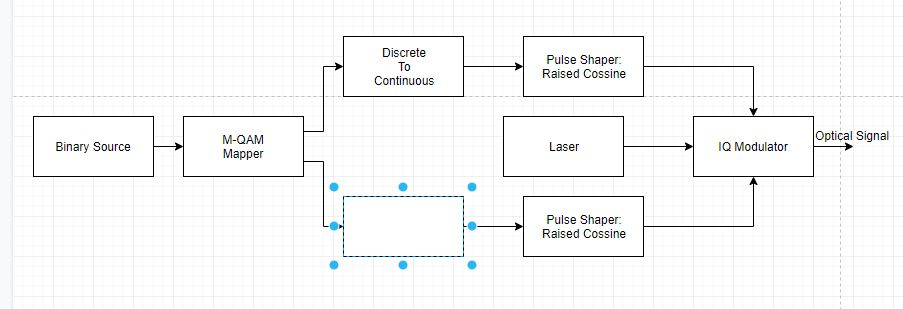
\includegraphics[scale=0.6]{../lib/m_qam_transmitter/figures/Transmitter_diagram.png}
	\caption{M-QAM Transmitter block diagram}
	\label{fig:trasmitter diagram}
\end{figure}

\begin{figure}[H]
    \centering
    \begin{subfigure}{0.4\textwidth}
    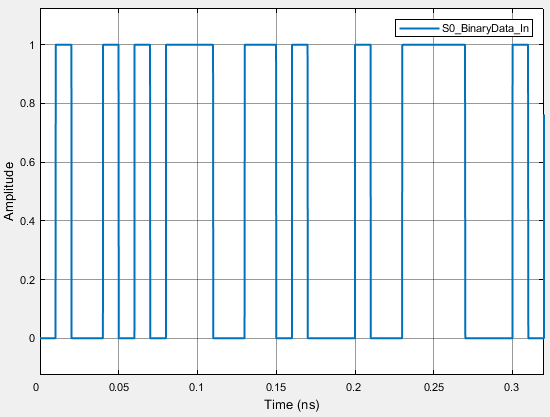
\includegraphics[scale=0.45]{../lib/m_qam_transmitter/figures/binary_in.png}
    \caption{Signal 0 Binary Source data}
    \label{fig:data}
    \end{subfigure}
    \begin{subfigure}{0.4\textwidth}
    	\centering
    	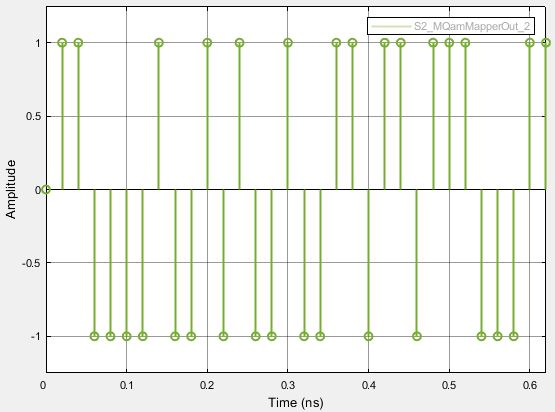
\includegraphics[scale=0.45]{../lib/m_qam_transmitter/figures/T_diracs.png}
    	\caption{Signal 1 Quadrature Mapper Out}
    	\label{fig:diracs}
	\end{subfigure}
\end{figure}
\begin{figure}[H]
    \centering
    \begin{subfigure}{0.4\textwidth}
    	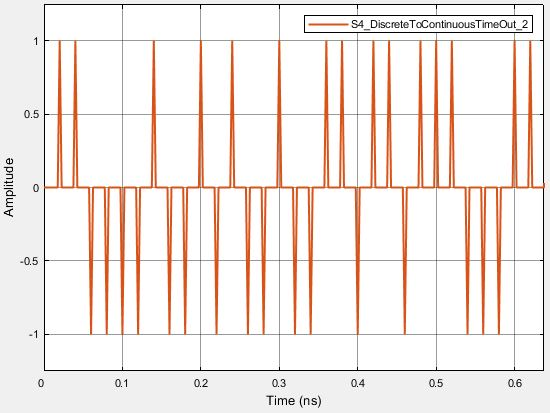
\includegraphics[scale=0.45]{../lib/m_qam_transmitter/figures/T_continuous_dirac.png}
    	\caption{signal 3 Discrete to Continous}
    	\label{fig:disc2Cont}
    \end{subfigure}
    \begin{subfigure}{0.4\textwidth}
    	\centering
    	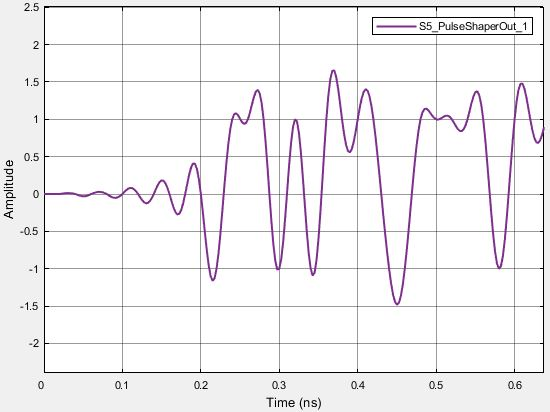
\includegraphics[scale=0.45]{./lib/m_qam_transmitter/figures/T_raised_cossine.png}
    	\caption{Signal 5 Pulse Shaper Out}
    	\label{fig:pulse shape}
    \end{subfigure}
\end{figure}

\begin{figure}[H]
    \centering
    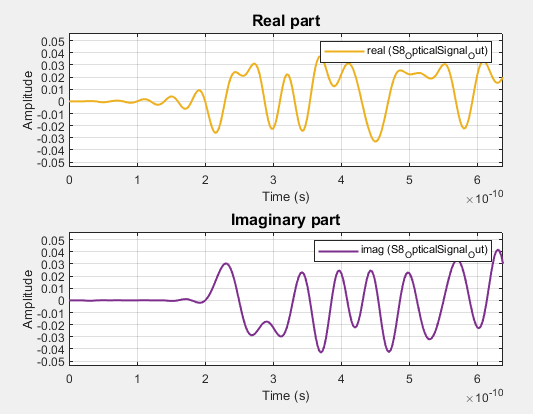
\includegraphics{../lib/m_qam_transmitter/figures/optical_out.png}
    \caption{Signal 8 IQ modulator Out}
    \label{fig:opticalOut}
\end{figure}

\begin{figure}[H]
	\centering
	\begin{subfigure}{0.4\textwidth}
		\centering
		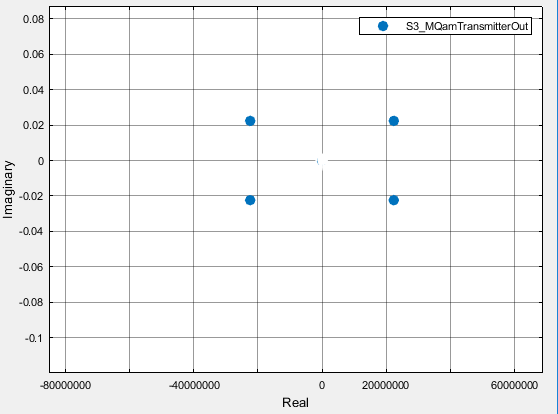
\includegraphics[scale=0.5]{./lib/m_qam_transmitter/figures/constellation_og.png}
		\caption{Original Constellation with a BER of 0}
		\label{fig:const_og}
	\end{subfigure}
	\begin{subfigure}{.4\textwidth}
		\centering
		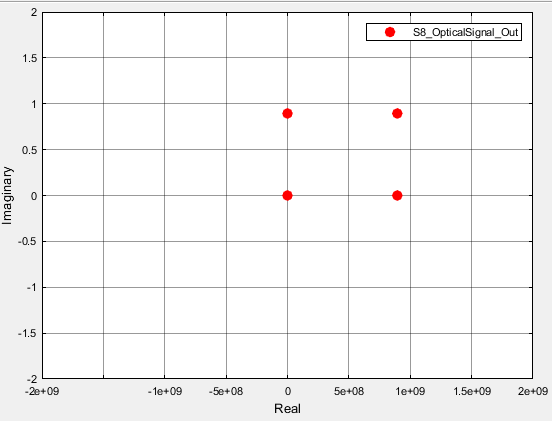
\includegraphics[scale=0.45]{./lib/m_qam_transmitter/figures/constellation2.png}
		\caption{Transladation of the original constellation with a BER of 0.22}
		\label{fig:const_new}
	\end{subfigure}
	\caption{Different constellations to test the noise impact}
	\label{fig:Constellations}
\end{figure}
\begin{figure}[H]
	\centering
	\begin{subfigure}{0.4\textwidth}
		\centering
		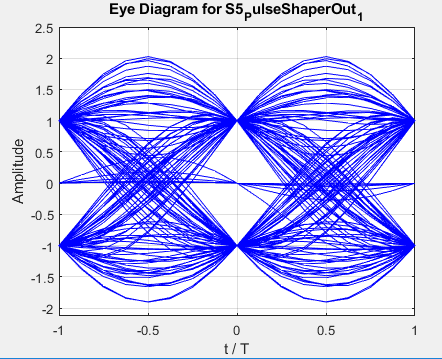
\includegraphics[scale=0.4]{./lib/m_qam_transmitter/figures/eye_no_noise.png}
		\caption{Eye diagram for the pulse shaper output}
		\label{fig:eye_clear}
	\end{subfigure}
	\begin{subfigure}{0.4\textwidth}
		\centering
		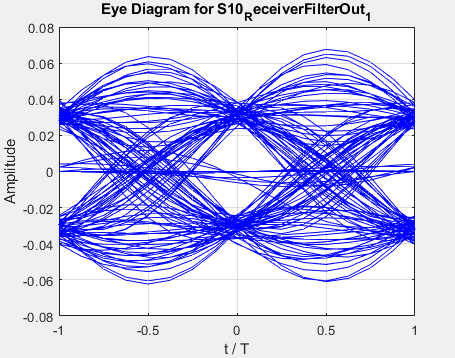
\includegraphics[scale=0.4]{./lib/m_qam_transmitter/figures/eye_noise.png}
		\caption{The eye diagram after we introduce noise in the receiver}
		\label{fig:eye_with_noise}
	\end{subfigure}
\caption{ISI interference}
\label{fig:eyes}
\end{figure}
\begin{figure}[H]
	\centering
	\begin{subfigure}{.4\textwidth}
		\centering
		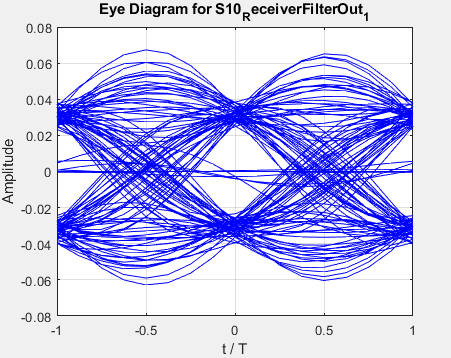
\includegraphics[scale=0.55]{./lib/m_qam_transmitter/figures/eye_noise_rolloff01.png}	
		\caption{Noise impact with a rolloff factor of 0.1}
		\label{fig:noise_roll01}
	\end{subfigure}
	\begin{subfigure}{.4\textwidth}
		\centering
		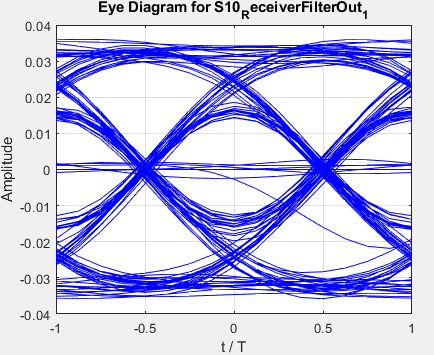
\includegraphics[scale=0.6]{./lib/m_qam_transmitter/figures/eye_noise_rolloff1.png}
		\caption{Noise impact with rolloff factor of 1}
		\label{fig:noise_roll1}	
	\end{subfigure}
\caption{The impact of noise on different rolloff factors}
\label{fig:noise_roll}	
\end{figure}
\begin{figure}[H]
	\centering
	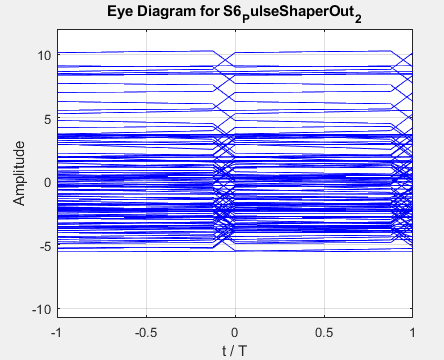
\includegraphics[scale=0.6]{./lib/m_qam_transmitter/figures/gaussian_shaper.png}
	\caption{The Gaussian pulse shaper eye diagram}
	\label{fig:gaussian}
\end{figure}
\pagebreak


\subsection*{Functional description}

\begin{text}
As we can see in \ref{fig:trasmitter diagram} the binary source generates random bits(\ref{fig:data}) that will be mapped by the \textit{M-QAM Mapper} according to the constellation. This mapper generates a dirac with variable amplitudes(\ref{fig:diracs}) which will be converted to a time continuous pulse(\ref{fig:disc2Cont}).\newline
This pulse will be shaped in raised cosine format in order to remove the inter-symbol interference as we can see in \ref{fig:pulse shape}. Thus, this signal will be modulated by the carrier by the \textit{IQ Modulator}.\newline
Since this type of modulation requires two carriers, one in quadrature and other in phase separated by 90\textdegree  in order to be orthogonal, we have two branches to do the respective modulation.\newline
The optical signal generated by the \textit{IQ Modulator} will then be propagated in the optical fiber.
\bigbreak
This type of modulation allow us to modify different aspects of the blocks, as an example, we can modify the rolloff factor of the raised cosine filter or even change the constellation. This modifications bring different results in the BER, Eye Diagram, etc. We will see the impact of changing the constellation and not having a infinite response pulse shaper.%tambem ver impacto do codigo de gray
\subsubsection{Impact of constellation and coding}
The default constellation is a square with amplitude unitary. We can change the format by changing the \textit{iqAmplitudes} vector in the library \textit{MQamMapper}. This has direct impact in the BER because we can modify the distance between symbols and consequently vary the Probability of error, as we can see in \ref{fig:Constellations}
In order to obtain the best BER values we must choose a balanced geometric shape.
\bigbreak
The assignment of bits to a symbol must be chosen carefully because if we have two symbols close in distance and between them the hamming distance is maximum, or in other words, we can read wrong all bits just because one block of the receiver injected noise into one of the carriers. If the bits defined to the symbol in the second quadrant were \textit{"11"} the BER would increase to practicaly 0.5.
\subsubsection{The pulse shaper}
We can choose between raised cosine, gaussian and root raised cosine and this type of impulse has the perk of having zero interference between symbols. In the other hand, this pulse shaping format has an infinite response and since we cant represent this on a real discrete system we must implement a \textit{FIR filter}.\newline
The impact of this filter depends on the number of impulses we define a, if we want better spectral efficiency we choose high order FIR filter.\newline
The bandwidth of the ouput signal of the pulse shaper is $ \frac{1}{T\textunderscore symbol}(1 + \beta) $ in which beta is the rolloff factor.\newline
When we add some noise into the receiver we expect to see some interference between symbols. In the \ref{fig:eyes} it is possible to see the differences in the \textit{ISI}. We can also conclude that the rolloff factor impacts the symbol interference(\ref{fig:noise_roll}) when we add noise to the system because the BER is dependent on the bandwidth of the signal and since a lower rolloff factor means lower bandwidth we will have less noise power.
\end{text}
\subsection{Open Issues}
\begin{text}
	The square filter type on the pulse shaper function it's not working
\end{text}
\subsection*{Sugestions for future improvement}
%pulse shaper squared dont work
